\subsection{Game V1}
As seen in Table \ref{tab:game-rules}, the game V1 rules are heavily stacked in favour of the prey. The effect of this can be seen in all of the fitness over time graphs that were produced. Even the experiments that included charged particles performed poorly with this version of the game. An example of a graph from experiments 1 and 17 can be seen in Figure \ref{fig:v1-no-charged-graphs} and an example of a graph from experiment 4 and 20 can be seen in Figure \ref{fig:v1-fully-charged-graphs}. In Figure \ref{fig:v1-fully-charged-graphs} it is expected that at least one particle should have a high fitness value, but as it can be seen, the full charged swarms from experiment 4 and 20 do not perform better than those from experiments 1 and 17.

\begin{figure}
  \centering
  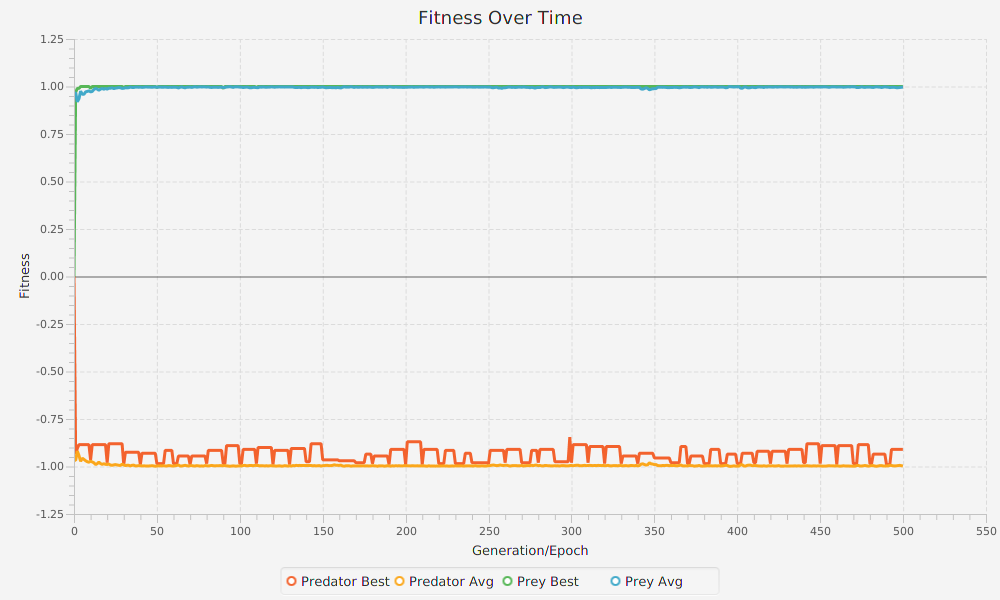
\includegraphics[width=0.7\textwidth]{exp25-Run-4.png}  
  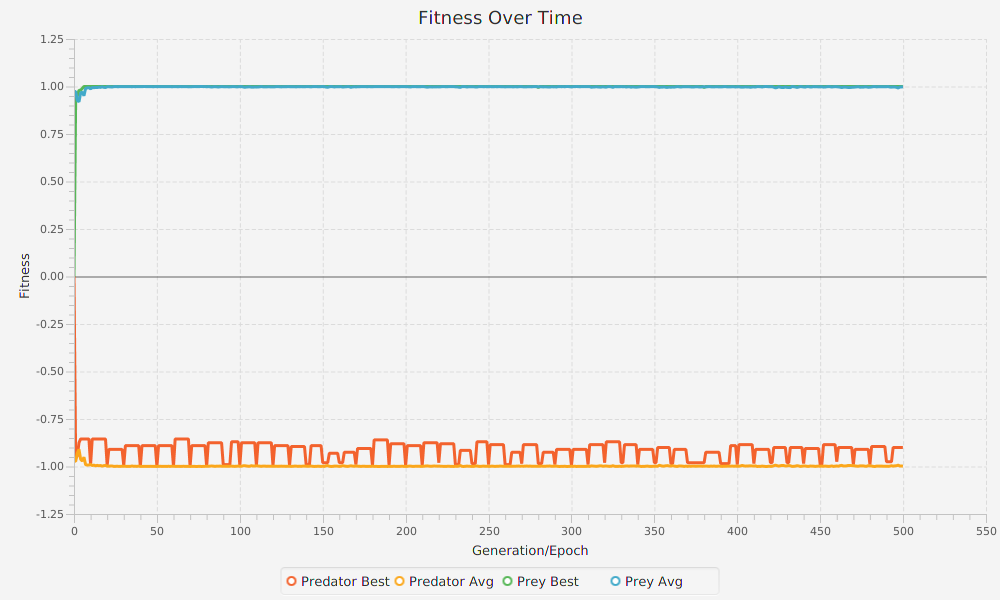
\includegraphics[width=0.7\textwidth]{exp41-Run-0.png}
  \caption{Game V1 Experiments 1(top) and 17(bottom)}
  \label{fig:v1-no-charged-graphs}
\end{figure}


\begin{figure}
  \centering
  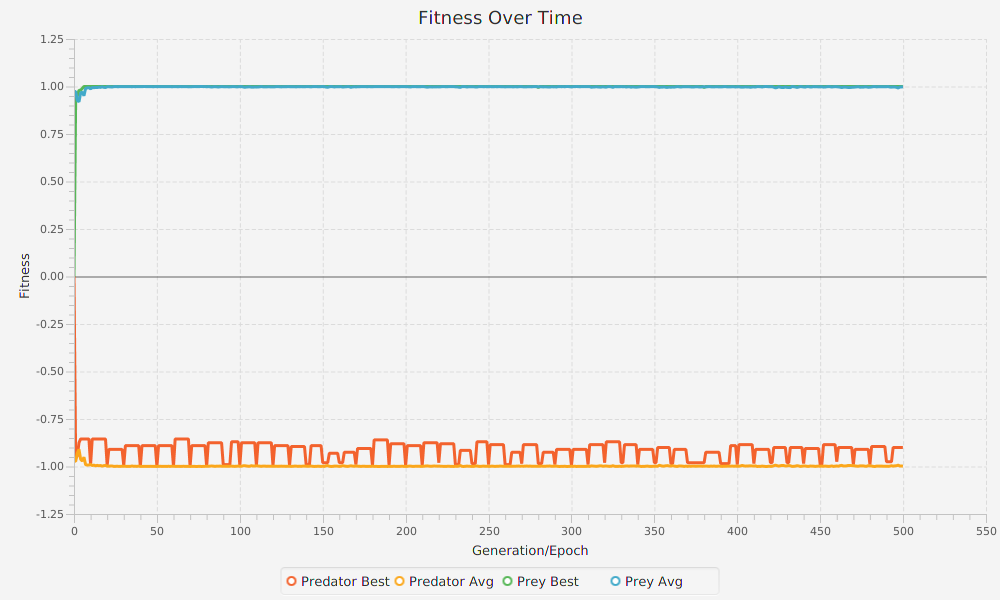
\includegraphics[width=0.7\textwidth]{exp28-Run-0.png}  
  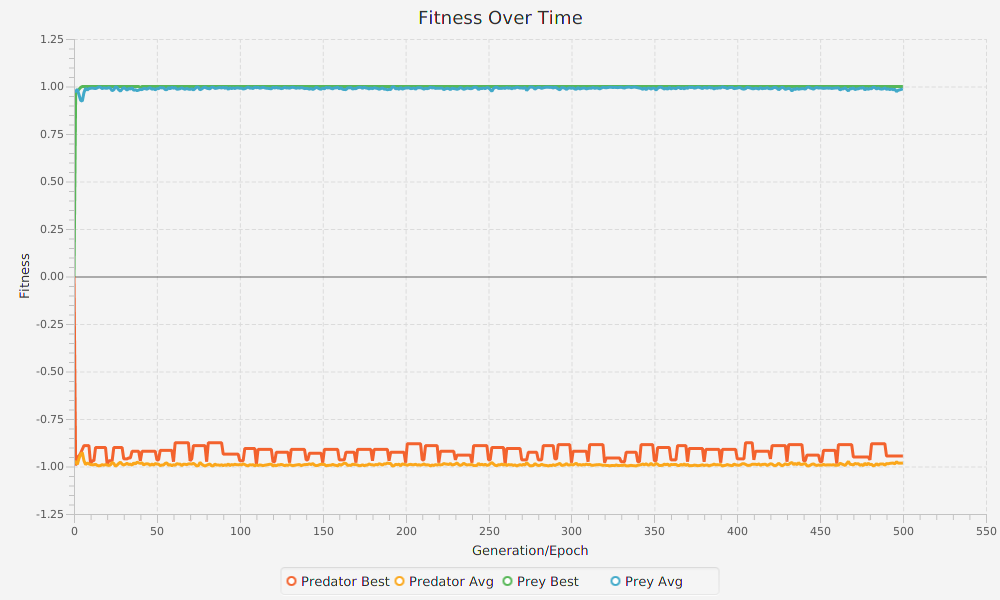
\includegraphics[width=0.7\textwidth]{exp44-Run-2.png}
  \caption{Game V1 Experiments 4(top) and 21(bottom)}
  \label{fig:v1-fully-charged-graphs}
\end{figure}

When observing the games being played by the particle with the best fitness over all of the runs an interesting pattern emerges. In most cases, the game ends with the prey running off of the board. This is because the easiest way for the prey to win if for it to fall off. While the predator also falls off about one third of the time, the predator tends to stay on the board for a longer time than the prey. An example of this technique can be seen in Figure \ref{fig:exp1-pred-game-58}. Observing the prey behaviour, this can be reinforced as the best prey had 324 games of 400 ending with the prey falling off the board. An example of several games can be seen in Figure \ref{fig:exp1-prey-example-games}. Unfortunately, since it is extremely easy for the prey to win and for the predator to lose, the type of behaviour that evolved is quite basic. In general, both agents tend to just move in a straight line until one of them falls off the board.


\begin{figure}
  \centering
  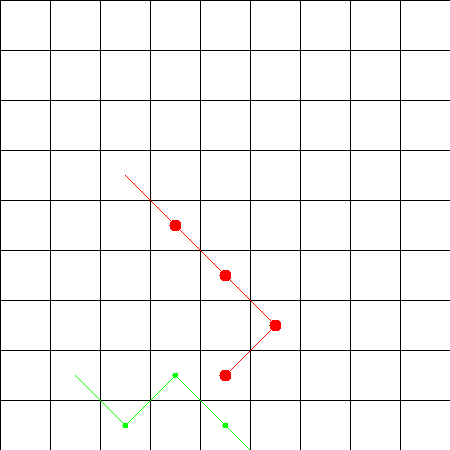
\includegraphics[width=0.5\textwidth]{exp25-pred-Game-382.png}
  \caption{Game V1 Experiment 1: Example predator game}
  \label{fig:exp1-pred-game-58}
\end{figure}

\begin{figure}
  \centering
  \begin{subfigure}{.4\textwidth}
  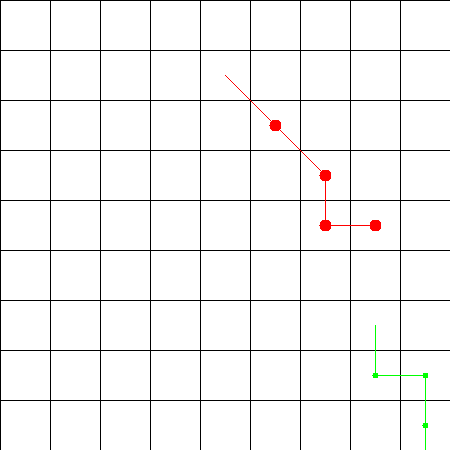
\includegraphics[width=\linewidth]{exp25-prey-Game-58.png}
  \end{subfigure}
  \begin{subfigure}{.4\textwidth}
  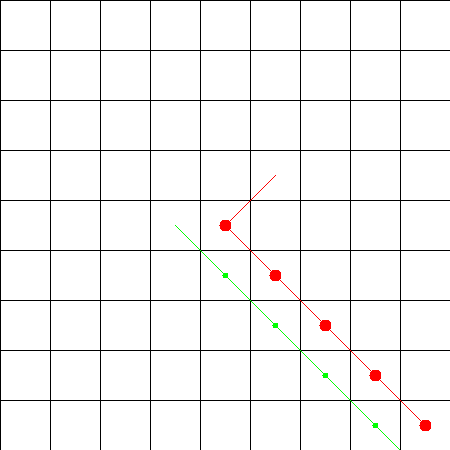
\includegraphics[width=\linewidth]{exp25-prey-Game-119.png}
  \end{subfigure} \\\hfill
  
  \begin{subfigure}{.4\textwidth}
   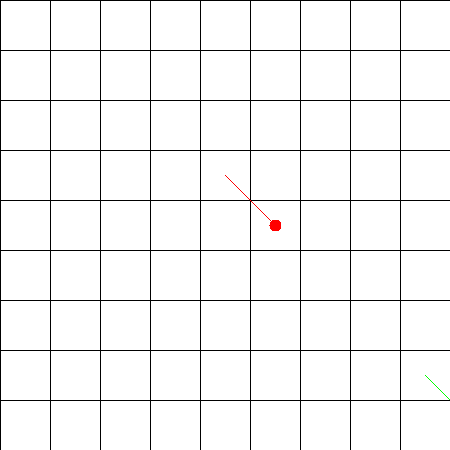
\includegraphics[width=\linewidth]{exp25-prey-Game-376.png}  
   \end{subfigure}
   \begin{subfigure}{.4\textwidth}
   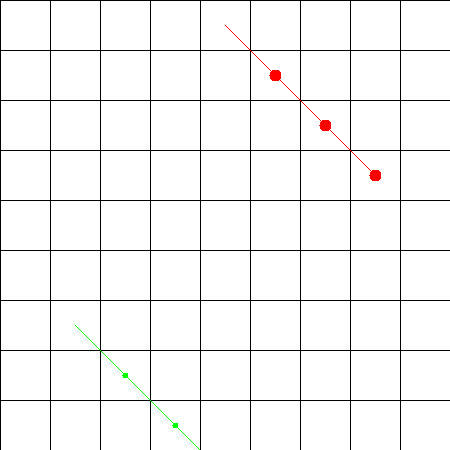
\includegraphics[width=\linewidth]{exp25-prey-Game-386.png}
   \end{subfigure}
  \caption{Game V1 Experiment 1: Examples of prey games \label{fig:exp1-prey-example-games}}
  
\end{figure}

\begin{table}
  \centering
  \begin{tabular}{|c|c|c|c|c|c|c|}
    \hline
    \multirow{2}{*}{Experiment} & \multicolumn{3}{|c|}{Predator} & \multicolumn{3}{|c|}{Prey} \\\cline{2-7}
    & Max & Average & Min & Max & Average & Min\\
    \hline
    1 & -0.845 & -0.875 & -0.900 & 1.000 & 1.000 & 0.999 \\
2 & -0.815 & -0.854 & -0.875 & 1.000 & 0.999 & 0.997 \\
3 & -0.845 & -0.870 & -0.890 & 1.000 & 0.998 & 0.996 \\
4 & -0.860 & -0.879 & -0.915 & 1.000 & 0.998 & 0.996 \\
5 & -0.835 & -0.868 & -0.920 & 1.000 & 1.000 & 0.998 \\
6 & -0.850 & -0.868 & -0.905 & 1.000 & 0.999 & 0.997 \\
7 & -0.850 & -0.876 & -0.915 & 1.000 & 0.998 & 0.995 \\
8 & -0.885 & -0.898 & -0.905 & 1.000 & 0.997 & 0.992 \\
9 & -0.865 & -0.884 & -0.905 & 1.000 & 0.999 & 0.998 \\
10 & -0.800 & -0.874 & -0.905 & 1.000 & 0.999 & 0.998 \\
11 & -0.840 & -0.867 & -0.895 & 1.000 & 0.997 & 0.995 \\
12 & -0.870 & -0.877 & -0.885 & 0.998 & 0.996 & 0.994 \\
13 & -0.850 & -0.871 & -0.905 & 1.000 & 0.999 & 0.998 \\
14 & -0.820 & -0.877 & -0.900 & 1.000 & 1.000 & 1.000 \\
15 & -0.835 & -0.877 & -0.900 & 1.000 & 0.999 & 0.997 \\
16 & -0.850 & -0.888 & -0.910 & 1.000 & 0.999 & 0.995 \\
17 & -0.855 & -0.875 & -0.915 & 1.000 & 1.000 & 0.999 \\
18 & -0.855 & -0.890 & -0.910 & 1.000 & 1.000 & 0.999 \\
19 & -0.840 & -0.869 & -0.905 & 1.000 & 0.999 & 0.998 \\
20 & -0.855 & -0.882 & -0.905 & 0.999 & 0.998 & 0.996 \\
21 & -0.845 & -0.874 & -0.900 & 1.000 & 1.000 & 1.000 \\
22 & -0.790 & -0.830 & -0.895 & 1.000 & 0.999 & 0.998 \\
23 & -0.815 & -0.854 & -0.880 & 1.000 & 0.999 & 0.999 \\
24 & -0.810 & -0.882 & -0.920 & 1.000 & 0.998 & 0.995\\
\hline
  \end{tabular}
  \caption{Game V1 Summary }
  \label{tab:v1-summary}
\end{table}



